% Nut thread wear against flight hours, with the inspection opportunities that existed.
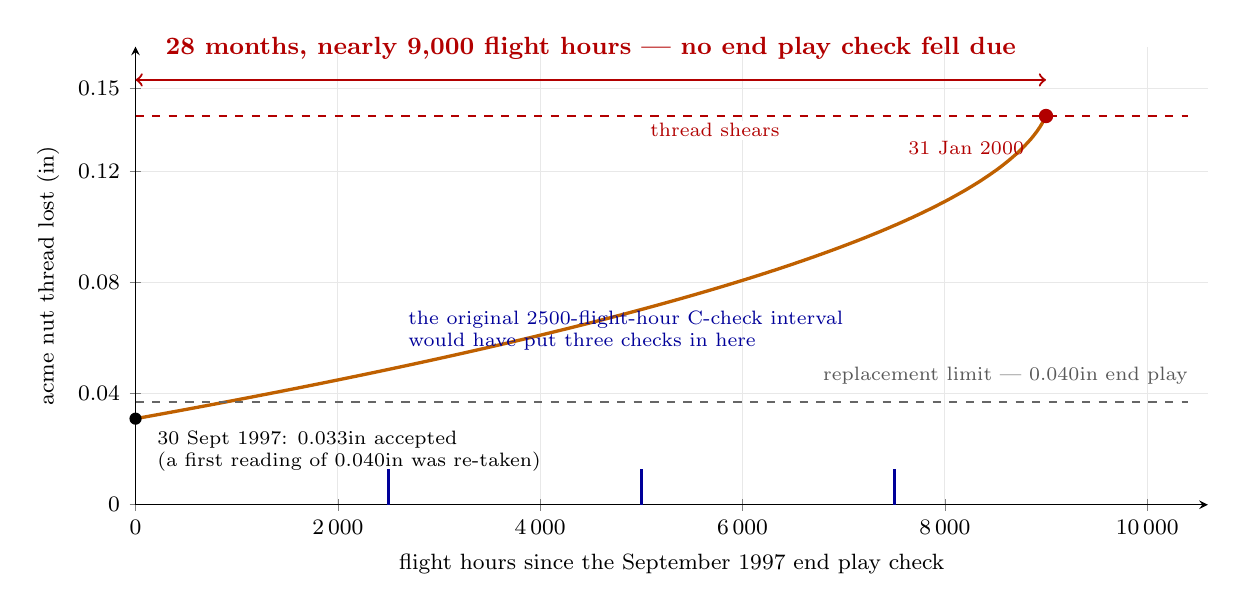
\begin{tikzpicture}
\begin{axis}[
  width=15.2cm,height=7.4cm,
  xlabel={flight hours since the September 1997 end play check},
  ylabel={acme nut thread lost (in)},
  xmin=0,xmax=10600,ymin=0,ymax=0.165,
  xtick={0,2000,4000,6000,8000,10000},
  scaled x ticks=false,
  xticklabel style={/pgf/number format/fixed,/pgf/number format/1000 sep={\,}},
  ytick={0,0.04,0.08,0.12,0.15},
  yticklabel style={/pgf/number format/fixed,/pgf/number format/precision=2},
  label style={font=\footnotesize},tick label style={font=\footnotesize},
  grid=both,grid style={gray!18},
  axis lines=left,clip=false]

% ---- the wear curve: Archard with p ~ 1/t gives t^2 linear in N ----
% starts at 0.031 in already lost, reaches 0.140 in at 9000 FH
\addplot[very thick,orange!75!black,domain=0:9000,samples=300]
  {0.15 - sqrt( (0.15-0.031)^2 - ((0.15-0.031)^2-(0.15-0.140)^2)*x/9000 )};

% ---- the two levels that matter ----
\draw[dashed,black!60] (axis cs:0,0.037) -- (axis cs:10400,0.037);
\node[font=\scriptsize,anchor=south west,text=black!65] at (axis cs:6700,0.040)
  {replacement limit --- \SI{0.040}{in} end play};
\draw[dashed,red!70!black,thick] (axis cs:0,0.140) -- (axis cs:10400,0.140);
\node[font=\scriptsize,anchor=north east,text=red!70!black,fill=white,inner sep=1pt]
  at (axis cs:6400,0.1385) {thread shears};

% ---- where it started ----
\fill[black] (axis cs:0,0.031) circle (2.2pt);
\node[font=\scriptsize,anchor=north west,align=left] at (axis cs:120,0.030)
  {30 Sept 1997: \SI{0.033}{in} accepted\\ \scriptsize(a first reading of \SI{0.040}{in} was re-taken)};

% ---- the accident ----
\fill[red!70!black] (axis cs:9000,0.140) circle (2.6pt);
\node[font=\scriptsize,anchor=north east,text=red!70!black,align=right]
  at (axis cs:8880,0.1345) {31 Jan 2000};

% ---- the span with no end play check due ----
\draw[<->,red!70!black,thick] (axis cs:0,0.153) -- (axis cs:9000,0.153);
\node[font=\small\bfseries,text=red!70!black,anchor=south]
  at (axis cs:4500,0.157) {28 months, nearly 9{,}000 flight hours --- no end play check fell due};

% ---- what the original interval would have given ----
\draw[blue!60!black,very thick] (axis cs:2500,0) -- (axis cs:2500,0.013);
\draw[blue!60!black,very thick] (axis cs:5000,0) -- (axis cs:5000,0.013);
\draw[blue!60!black,very thick] (axis cs:7500,0) -- (axis cs:7500,0.013);
\node[font=\scriptsize,text=blue!60!black,anchor=south west,align=left]
  at (axis cs:2600,0.052)
  {the original \mbox{2500-flight-hour} C-check interval\\ would have put three checks in here};

\end{axis}
\end{tikzpicture}
